\section{Testes}
Nos testes da aplicação, foram desenvolvidos scripts de testes ponta a ponta automatizados utilizando o Cypress. Esta metodologia foi escolhida, pois, com ela, é possível testar todos os elementos da aplicação simulando o ambiente real. 

Nesta seção, serão apresentados os casos de testes implementados bem como os resultados parciais de sua execução.


\subsection{Cadastro de Escolas}
A \autoref{fig:teste-escola} mostra os casos de testes implementados para a entidade Escola da aplicação. O fluxo dos testes se inicia com o acesso na aplicação através de um usuário com o perfil administrador; em seguida é acessado o painel de escolas e nele é realizado o cadastro, alteração de uma escola.

\begin{figure}[htb]
    \centering
	
\includegraphics[width=16cm]{imagens/tstEscola.JPG}
	\caption{\label{fig:teste-escola} Casos de testes do cadastro de escolas.}
	\fonte{Os autores}
\end{figure}

\subsection{Cadastro de Usuários}
A \autoref{fig:teste-admin} mostra os casos de testes implementados para usuários com o perfil de administrador. O fluxo desse teste se inicia com o acesso na aplicação através de um usuário com o perfil administrador; em seguida é acessado o painel de usuários e nele é realizado o cadastro, alteração e um usuário

\begin{figure}[htb]
    \centering
	
\includegraphics[width=16cm]{imagens/tstAdmin.JPG}
	\caption{\label{fig:teste-admin} Casos de testes do cadastro de administradores.}
	\fonte{Os autores}
\end{figure}

\subsection{Cadastro de Gestores}
A \autoref{fig:teste-gestor} mostra os casos de testes implementados para usuários com o perfil Gestor. O fluxo desse teste se inicia com o acesso na aplicação através de um usuário com o perfil administrador; em seguida é acessado o painel de gestores e nele é realizado o cadastro, alteração de um gestor

\begin{figure}[htb]
    \centering
	
\includegraphics[width=16cm]{imagens/tstGestor.JPG}
	\caption{\label{fig:teste-gestor} Casos de testes do cadastro de gestores.}
	\fonte{Os autores}
\end{figure}

\subsection{Cadastro de Professores}
A \autoref{fig:teste-professor} mostra os casos de testes implementados para usuários com o perfil Professor. O fluxo desse teste se inicia com o acesso na aplicação através de um usuário com o perfil gestor; em seguida é acessado o painel de gestores e nele é realizado o cadastro, alteração de um professor.

\begin{figure}[htb]
    \centering
	
\includegraphics[width=16cm]{imagens/tstProfessor.JPG}
	\caption{\label{fig:teste-professor} Casos de testes do cadastro de professores.}
	\fonte{Os autores}
\end{figure}

\subsection{Cadastro de Alunos}
A \autoref{fig:teste-aluno} mostra os casos de testes implementados para usuários com o perfil Aluno. O fluxo desse teste se inicia com o acesso na aplicação através de um usuário com o perfil gestor; em seguida é acessado o painel de alunos e nele é realizado o cadastro, alteração de um aluno.

\begin{figure}[htb]
    \centering
	
\includegraphics[width=16cm]{imagens/tstAluno.JPG}
	\caption{\label{fig:teste-aluno} Casos de testes do cadastro de alunos.}
	\fonte{Os autores}
\end{figure}

\subsection{Cadastro de Turmas}
A \autoref{fig:teste-turma} mostra os casos de testes implementados para o cadastro de turmas. O fluxo desse teste se inicia com o acesso na aplicação através de um usuário com o perfil gestor; em seguida é acessado o painel de turmas onde é realizado o cadastro, alteração de um aluno.

\begin{figure}[htb]
    \centering
	
\includegraphics[width=16cm]{imagens/tstTurma.JPG}
	\caption{\label{fig:teste-turma} Casos de testes do cadastro de turmas.}
	\fonte{Os autores}
\end{figure}

\subsection{Cadastro de Conquistas}
A \autoref{fig:teste-conquista} mostra os casos de testes implementados para as conquistas. O fluxo desse teste se inicia com o acesso na aplicação através de um usuário com o perfil de professor e em seguida acessando o painel de  conquistas para realização do cadastro e alteração. 

\begin{figure}[htb]
    \centering
	
\includegraphics[width=16cm]{imagens/tstConquista.JPG}
	\caption{\label{fig:teste-conquista} Casos de testes do cadastro de conquistas.}
	\fonte{Os autores}
\end{figure}

\subsection{Cobertura de código}

A \autoref{fig:teste-backend} representa o resultado dos testes no \textit{\gls{back-end}}. Com isso, pode-se notar que a cobertura média da aplicação ficou em torno de 40\%, uma nota abaixo do esperado, porém isso aconteceu devido ao curto período de tempo disponível para o desenvolvimento do projeto.
\begin{figure}[htb]
    \centering
	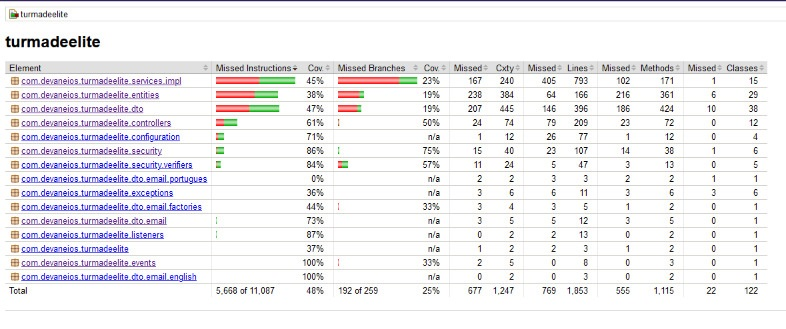
\includegraphics[width=16cm]{imagens/TesteBackend.jpg}
	\caption{\label{fig:teste-backend} Resultado dos testes no back-end.}
	\fonte{Os autores}
\end{figure}

Já no \textit{\gls{front-end}}, após a execução dos testes implementados, foi alcançado o nível de cobertura de código apresentado na \autoref{fig:cobetura}.

\begin{figure}[htb]
    \centering
	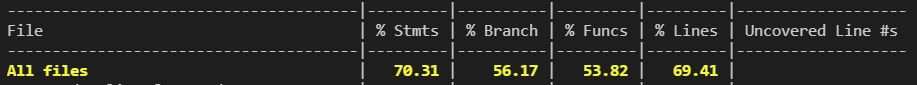
\includegraphics[width=16cm]{imagens/ResultadoTestes.JPG}
	\caption{\label{fig:cobetura} Cobertura de código}
	\fonte{Os autores}
\end{figure}

No geral, os testes no \textit{\gls{front-end}} cobriram 69.41\% das linhas de código, uma  porcentagem não suficiente devido ao tempo curto para o desenvolvimento do projeto.
